\documentclass{article}
\usepackage[utf8]{inputenc}

\title{Knuth's Dancing Links}
\author{Oisín Hodgins, Seán Monahan }
\date{NUIG Final Year Project (Mathematics)}
\usepackage{natbib}
\usepackage[table, svgnames, dvipsnames, array]{xcolor}
\usepackage{graphicx}
\usepackage{tikz}
\usepackage{colortbl}
\usepackage{amsmath}
\usepackage{nccmath}
\usepackage{algorithm}
\usepackage[noend]{algpseudocode}
\usepackage{soul}
\def\checkmark{\tikz\fill[scale=0.4](0,.35) -- (.25,0) -- (1,.7) -- (.25,.15) -- cycle;}
\makeatletter
\def\BState{\State\hskip-\ALG@thistlm}
\makeatother

\begin{document}

\maketitle
\clearpage
\section{Declaration page}
\clearpage
\section{Introduction}
Donald Knuth is seen as the founder of many aspects of modern computer science, often considered the "father of analysis of algorithms". Even the typeset that this project is written in, \LaTeX, is built using the \TeX{} system developed by Knuth. Our motivation for this project is to gain some insight into how the field of computer science developed in to what it is today, with credit to Knuth's vast list of  contributions. In this report, we will be looking at his \textit{Dancing Links} technique used in conjunction with \textit{Algorithm X} from \cite{dlx}. It's a fascinating case where a simple operation, which was overlooked by most programmers at the time, improved the solving time for Exact Cover problem implementations immensely. In this introduction we aim to gain some insight in to what an exact cover problem is and break down its essence using a motivating example.

\subsection{The Exact Cover Problem}
Given a set $X$, and a collection of its subsets $S$, an \textbf{exact cover} is the sub-collection $S^*$ of $S$ in which each element of ${X}$ appears in exactly one subset of $S^*$. In an \textbf{exact cover problem} we are concerned with determining whether an exact cover exists. The most famous examples of exact cover problems include Sudoku and the N-Queens problem which we will see later, but first let's consider a Latin Square to help illustrate what is meant by an exact cover problem.\\ 
\subsection{Latin Square Problem}

\begin{center}
\begin{tabular}{cccc}
 & 0 & 1 & 2\\ \cline{2-4} 
\multicolumn{1}{c|}{0} & \multicolumn{1}{c|}{$A$} & \multicolumn{1}{c|}{$B$}& \multicolumn{1}{c|}{$C$} \\ \cline{2-4} 
\multicolumn{1}{c|}{1} & \multicolumn{1}{c|}{$B$} & \multicolumn{1}{c|}{$C$}& \multicolumn{1}{c|}{$A$} \\ \cline{2-4} 
\multicolumn{1}{c|}{2} & \multicolumn{1}{c|}{$C$} & \multicolumn{1}{c|}{$A$}& \multicolumn{1}{c|}{$B$} \\ \cline{2-4} 
\end{tabular}

\end{center}
A Latin Square is a puzzle similar to Sudoku that was inspired by Leonard Euler, where an $N$X$N$ grid must be filled with $N$ distinct shapes, such that no two identical shapes share the same column or row. Here we include notation that denotes where each symbol $A$, $B$, $C$ lie, i.e. in above 3X3 example, $A$ lies at $(0,0)$ and $(1,2)$ and $(2,1)$. As an example we will construct a simple 2X2 Latin Square, posing the puzzle as an Exact Cover Problem. The grid below illustrates the $2X2$ grid including coordinates before any symbols are placed.
\begin{center}
\begin{tabular}{ccc}
 & 0 & 1 \\ \cline{2-3} 
\multicolumn{1}{c|}{0} & \multicolumn{1}{c|}{} & \multicolumn{1}{c|}{} \\ \cline{2-3} 
\multicolumn{1}{c|}{1} & \multicolumn{1}{c|}{} & \multicolumn{1}{c|}{} \\ \cline{2-3} 
\end{tabular}
\end{center}
Let's break down the \textbf{constraints} of the 2X2 puzzle, where $C_i$ refers to the numbering of the constraint.\\
First, we consider the fact that each square in the grid needs a \textbf{symbol}:\\
$C_1$ :  (0,0) must have a symbol\\
$C_2$ :  (0,1) must have a symbol\\
$C_3$ :  (1,0) must have a symbol\\
$C_4$ :  (1,1) must have a symbol\\
Next we consider the \textbf{row constraint}:\\
$C_5$ :  Symbol A must appear in row 0\\
$C_6$ :  Symbol B must appear in row 0\\
$C_7$ :  Symbol A must appear in row 1\\
$C_8$ :  Symbol B must appear in row 1\\
Finally we consider the \textbf{column constraint},\\
$C_9$ :  Symbol A must appear in column 0\\
$C_{10}$ :  Symbol B must appear in column 0\\
$C_{11}$ :  Symbol A must appear in column 1\\
$C_{12}$ :  Symbol B must appear in column 1\\
These are our 12 constraints for the puzzle. Now we can construct a checklist to that might help us solve the puzzle, where $C_i$ are the constraints, and S@(x,y) refers to the symbol at coordinates (x,y)\\\\
\renewcommand{\arraystretch}{2.5}
\begin{tabular}{ |p{1.25cm}|p{0.4cm}|p{0.4cm}|p{0.4cm}|p{0.4cm}|p{0.4cm}|p{0.4cm}|p{0.4cm}|p{0.4cm}|p{0.4cm}|p{0.4cm}|p{0.4cm}|p{0.4cm}|  }
 \rowcolor[rgb]{0.6,0.6,0.6}
& \multicolumn{12}{|c|}{Constraints} \\
 \hline
\rowcolor[rgb]{0.6,0.6,0.6}& $C_1$ & $C_2$ &  $C_3$ & $C_4$ & $C_5$ & $C_6$ & $C_7$ & $C_8$ & $C_9$ & $C_{10}$ &$C_{11}$ & $C_{12}$ \\ \hline
\rowcolor[rgb]{0.867,0.867,0.867}$A@(0,0)$ &  \textcolor{ForestGreen}{\checkmark}   & $\textcolor{red}{X}$   &$\textcolor{red}{X}$&$\textcolor{red}{X}$&$\textcolor{ForestGreen}{\checkmark}$ &  $\textcolor{red}{X}$   & $\textcolor{red}{X}$   &$\textcolor{red}{X}$&$\textcolor{ForestGreen}{\checkmark}$&$\textcolor{red}{X}$& $\textcolor{red}{X}$   &$\textcolor{red}{X}$\\ \hline
\rowcolor[rgb]{0.753,0.753,0.753}$A@(0,1)$ &  $\textcolor{red}{X}$   & $\textcolor{ForestGreen}{\checkmark}$   &$\textcolor{red}{X}$&$\textcolor{red}{X}$&$\textcolor{red}{X}$&  $\textcolor{ForestGreen}{\checkmark}$   & $\textcolor{red}{X}$   &$\textcolor{red}{X}$&$\textcolor{ForestGreen}{\checkmark}$&$\textcolor{red}{X}$  & $\textcolor{red}{X}$   &$\textcolor{red}{X}$\\ \hline
\rowcolor[rgb]{0.867,0.867,0.867}  $A@(1,0)$    &  $\textcolor{red}{X}$   &$\textcolor{red}{X}$   &$\textcolor{ForestGreen}{\checkmark}$&$\textcolor{red}{X}$&$\textcolor{ForestGreen}{\checkmark}$ &  $\textcolor{red}{X}$   & $\textcolor{red}{X}$  &$\textcolor{red}{X}$&$\textcolor{red}{X}$&$\textcolor{ForestGreen}{\checkmark}$ &$\textcolor{red}{X}$   &$\textcolor{red}{X}$\\ \hline
\rowcolor[rgb]{0.753,0.753,0.753}$A@(1,1)$    &  $\textcolor{red}{X}$   & $\textcolor{red}{X}$   &$\textcolor{red}{X}$&$\textcolor{ForestGreen}{\checkmark}$&$\textcolor{red}{X}$&  $\textcolor{ForestGreen}{\checkmark}$   & $\textcolor{red}{X}$   &$\textcolor{red}{X}$&$\textcolor{red}{X}$&$\textcolor{ForestGreen}{\checkmark}$& $\textcolor{red}{X}$   &$\textcolor{red}{X}$\\ \hline
\rowcolor[rgb]{0.867,0.867,0.867}  $B@(0,0)$  &  $\textcolor{ForestGreen}{\checkmark}$   & $\textcolor{red}{X}$   &$\textcolor{red}{X}$&$\textcolor{red}{X}$&$\textcolor{red}{X}$&  $\textcolor{red}{X}$   & $\textcolor{ForestGreen}{\checkmark}$   &$\textcolor{red}{X}$&$\textcolor{red}{X}$&$\textcolor{red}{X}$& $\textcolor{ForestGreen}{\checkmark}$   &$\textcolor{red}{X}$\\ \hline
\rowcolor[rgb]{0.753,0.753,0.753}$B@(0,1)$ &  $\textcolor{red}{X}$   & $\textcolor{ForestGreen}{\checkmark}$   &$\textcolor{red}{X}$&$\textcolor{red}{X}$&$\textcolor{red}{X}$&  $\textcolor{red}{X}$   & $\textcolor{red}{X}$   &$\textcolor{ForestGreen}{\checkmark}$&$\textcolor{red}{X}$&$\textcolor{red}{X}$& $\textcolor{ForestGreen}{\checkmark}$   &$\textcolor{red}{X}$\\ \hline
\rowcolor[rgb]{0.867,0.867,0.867}   $B@(1,0)$ &  $\textcolor{red}{X}$   & $\textcolor{red}{X}$   &$\textcolor{ForestGreen}{\checkmark}$&$\textcolor{red}{X}$&$\textcolor{red}{X}$&  $\textcolor{red}{X}$   & $\textcolor{ForestGreen}{\checkmark}$   &$\textcolor{red}{X}$&$\textcolor{red}{X}$&$\textcolor{red}{X}$& $\textcolor{red}{X}$   &$\textcolor{ForestGreen}{\checkmark}$\\ \hline
\rowcolor[rgb]{0.753,0.753,0.753} $B@(1,1)$ &  $\textcolor{red}{X}$   & $\textcolor{red}{X}$   &$\textcolor{red}{X}$&$\textcolor{ForestGreen}{\checkmark}$&$\textcolor{red}{X}$&  $\textcolor{red}{X}$   & $\textcolor{red}{X}$   &$\textcolor{ForestGreen}{\checkmark}$&$\textcolor{red}{X}$&$\textcolor{red}{X}$& $\textcolor{red}{X}$   &$\textcolor{ForestGreen}{\checkmark}$\\\hline
\end{tabular}
\newline
\newline 
\newline
Since we have our checklist with all necessary constraints and placements, we can directly construct a "One-Zero" matrix by simply changing $\textcolor{ForestGreen}{\checkmark}$ to ones and $\textcolor{red}{X}$ to zeros while retaining the $8X12$ shape of the table, which we will denote as $A$ for this example:\\
\begin{center}
\setcounter{MaxMatrixCols}{20}
\begin{math}
\LARGE{A}=
\small{
\begin{bmatrix}
&1 & 0 & 0 & 0 & 1 & 0 & 0 & 0 & 1 & 0 & 0 & 0 &\\
&0 & 1 & 0 & 0 & 0 & 1 & 0 & 0 & 1 & 0 & 0 & 0 &\\
&0 & 0 & 1 & 0 & 1 & 0 & 0 & 0 & 0 & 1 & 0 & 0 &\\
&0 & 0 & 0 & 1 & 0 & 1 & 0 & 0 & 0 & 1 & 0 & 0 &\\
&1 & 0 & 0 & 0 & 0 & 0 & 1 & 0 & 0 & 0 & 1 & 0 &\\
&0 & 1 & 0 & 0 & 0 & 0 & 0 & 1 & 0 & 0 & 1 & 0 &\\
&0 & 0 & 1 & 0 & 0 & 0 & 1 & 0 & 0 & 0 & 0 & 1 &\\
&0 & 0 & 0 & 1 & 0 & 0 & 0 & 1 & 0 & 0 & 0 & 1 &\\ 
\end{bmatrix}}
\end{math}
\end{center}
Now that we have our problem posed in a suitable format, let's venture into our goal, as Donald Knuth puts it:\\
“Given a matrix of 0s and 1s, does it have a set of rows containing exactly one 1 in each column?”
\cite{dlx}\\

\subsection{Solution to the Latin Square}
Deducing a solution using trial and error in this case is quite trivial since there are so few options, even without constructing A one might deduce the following solution:\\
\begin{center}
\begin{tabular}{ccc}
 & 0 & 1 \\ \cline{2-3} 
\multicolumn{1}{c|}{0} & \multicolumn{1}{c|}{$A$} & \multicolumn{1}{c|}{$B$} \\ \cline{2-3} 
\multicolumn{1}{c|}{1} & \multicolumn{1}{c|}{$B$} & \multicolumn{1}{c|}{$A$} \\ \cline{2-3} 
\end{tabular}
\end{center}
This gives us one possible solution with the following choices; A@(0,0), B@(0,1), B@(1,0), and A@(1,1). We can eliminate the other options in the table:\\
\renewcommand{\arraystretch}{2.5}
\begin{tabular}{ |p{1.25cm}|p{0.4cm}|p{0.4cm}|p{0.4cm}|p{0.4cm}|p{0.4cm}|p{0.4cm}|p{0.4cm}|p{0.4cm}|p{0.4cm}|p{0.4cm}|p{0.4cm}|p{0.4cm}|  }
 \rowcolor[rgb]{0.6,0.6,0.6}
& \multicolumn{12}{|c|}{Constraints} \\
 \hline
\rowcolor[rgb]{0.6,0.6,0.6}& $C_1$ & $C_2$ &  $C_3$ & $C_4$ & $C_5$ & $C_6$ & $C_7$ & $C_8$ & $C_9$ & $C_{10}$ & $C_{11}$ & $C_{12}$ \\ \hline
\rowcolor[rgb]{0.867,0.867,0.867}$A@(0,0)$ &  \textcolor{ForestGreen}{\checkmark}   & $\textcolor{red}{X}$   &$\textcolor{red}{X}$&$\textcolor{red}{X}$&$\textcolor{ForestGreen}{\checkmark}$ &  $\textcolor{red}{X}$   & $\textcolor{red}{X}$   &$\textcolor{red}{X}$&$\textcolor{ForestGreen}{\checkmark}$&$\textcolor{red}{X}$& $\textcolor{red}{X}$   &$\textcolor{red}{X}$\\ \hline
\rowcolor[rgb]{0.753,0.753,0.753}$A@(1,1)$    &  $\textcolor{red}{X}$   & $\textcolor{red}{X}$   &$\textcolor{red}{X}$&$\textcolor{ForestGreen}{\checkmark}$&$\textcolor{red}{X}$&  $\textcolor{ForestGreen}{\checkmark}$   & $\textcolor{red}{X}$   &$\textcolor{red}{X}$&$\textcolor{red}{X}$&$\textcolor{ForestGreen}{\checkmark}$& $\textcolor{red}{X}$   &$\textcolor{red}{X}$\\ \hline
\rowcolor[rgb]{0.867,0.867,0.867}$B@(0,1)$ &  $\textcolor{red}{X}$   & $\textcolor{ForestGreen}{\checkmark}$   &$\textcolor{red}{X}$&$\textcolor{red}{X}$&$\textcolor{red}{X}$&  $\textcolor{red}{X}$   & $\textcolor{red}{X}$   &$\textcolor{ForestGreen}{\checkmark}$&$\textcolor{red}{X}$&$\textcolor{red}{X}$& $\textcolor{ForestGreen}{\checkmark}$ &$\textcolor{red}{X}$\\ \hline
\rowcolor[rgb]{0.753,0.753,0.753}   $B@(1,0)$ &  $\textcolor{red}{X}$   & $\textcolor{red}{X}$   &$\textcolor{ForestGreen}{\checkmark}$&$\textcolor{red}{X}$&$\textcolor{red}{X}$&  $\textcolor{red}{X}$   & $\textcolor{ForestGreen}{\checkmark}$   &$\textcolor{red}{X}$&$\textcolor{red}{X}$&$\textcolor{red}{X}$& $\textcolor{red}{X}$   &$\textcolor{ForestGreen}{\checkmark}$\\ \hline
   
 \hline
\end{tabular}
\newline
\newline
Here we see the solution to the problem, where every constraint is filled exactly once. We can denote in matrix form as:\\
\begin{center}
\setcounter{MaxMatrixCols}{20}
\begin{math}
\LARGE{A^*}=
\small{
\begin{bmatrix}
&1 & 0 & 0 & 0 & 1 & 0 & 0 & 0 & 1 & 0 & 0 & 0 &\\
&0 & 0 & 0 & 1 & 0 & 1 & 0 & 0 & 0 & 1 & 0 & 0 &\\
&0 & 1 & 0 & 0 & 0 & 0 & 0 & 1 & 0 & 0 & 1 & 0 &\\
&0 & 0 & 1 & 0 & 0 & 0 & 1 & 0 & 0 & 0 & 0 & 1 &\\
\end{bmatrix}}
\end{math}
\end{center}
In $A^*$ we see exactly one 1 in every column. This satisfies Knuth's criteria for a solution to the Exact Cover Method but our method is not reliable. This was a very simple example where a trial and error approach gives us the answer quickly but in cases such as the N-Queens problem, for large N we have a much larger number of both choices (rows) at $N^2$ and constraints (columns) at $6*(N-1)$. In these less trivial cases the Exact Cover Problem are considered \textbf{NP-Complete}.\\

\clearpage
\section{Algorithm X and Dancing Links}
\subsection{NP-Complexity}
\textbf{Polynomial time} is a metric used to classify the complexity of a decision problem. An algorithm is said to be of polynomial time if its running time is upper bounded by a polynomial expression in the size of the input for the algorithm i.e., $T(n) = O(n^c)$ for some positive constant $c$. In other words, polynoimal time is a measure of the efficiency of the algorithm, which measures the growth of the number of operations relative to the size $n$ of the problem. \textbf{NP}, an abbreviation of "nondeterministic, polynomial time", refers to a problem that is solvable by a nondeterministic Turing Machine in polynomial time. Essentially, what we would need is a computer program which can output enough random "guesses" will be able to solve the problem within a realistic amount of time. An \textbf{NP-Complete} problem is one that upholds the definition of an NP problem, but can also be used for other problems with similar solvability. If the exact cover problem is NP-Complete, then if we can develop a nondeterministic algorithm that will find all solutions of one type of exact cover problem such as the Latin Square problem we saw in the previous section, it can solve any exact cover problem. In this project we will use Algorithm X using the Dancing Links technique developed by Donald Knuth to fulfill the requirements of an NP-Complete problem. % needs to be rewritten more clearly
[...] \\

\subsection{Why choose Algorithm X?}
Algorithm X a \textbf{nondeterministic}, \textbf{recursive}, \textbf{depth-first} \textbf{backtracking} algorithm used to find all solutions to the exact cover problem defined by any given matrix A of 0s and 1s. Before we go into the algorithm itself, let's review the definition and importance of these properties. \textbf{Nondeterministic} algorithms, given a particular input, will not always produce the same output. This is essential for an exact cover problem as the algorithm isn't restricted to finding only one solution. \textbf{Recursive} algorithms will rerun subroutines and functions until a specific condition is met, allowing efficiency by reusing a block of code until a solution is found. When incrementally building a solution, \textbf{backtracking} allows the algorithm to abandon a path that fails to meet the criteria. We will later look at what depth-first backtracking means, how it is implemented and how it improves efficiency.
\clearpage
\subsection{Algorithm X Pseudo-code}

\begin{itemize}
\item Let $A$ be the given one-zero matrix.
\item let $M$ be the set of unsatisfied columns. These are columns that have more than exactly one 1 in its rows.
\item let  $r_i$ and $c_j$ be the rows and columns of $A$, respectively, where $r_1$ is the first row, et cetera.
\end{itemize}

\begin{algorithm}
\caption{Algorithm X}\label{ax} 
\begin{algorithmic}[1]
\If{$M$ is empty}: the problem is solved \Return{$A$} \EndIf
\State Otherwise choose a  column $c$ from set $M$
\State Choose a row $r$ of $c$ that has value 1 (nondeterministically)
\For{each $j$ such that $A[r, j] = 1$}: \State{remove column $j$ from set $M$}
\ForAll{$i$ such that $A[i, j] = 1$}:\State{delete row $i$ from matrix $A$} \EndFor
\EndFor
\end{algorithmic}
\end{algorithm}
The algorithm works by methodically taking each unsatisfied constraint, randomly choosing one position that can fulfill its constraint and all removing other positions that have conflict with that constraint. Then we continue this process until a solution is found. This is implementation is slightly different to Knuth's which does not include $M$, this was added in for illustrative purposes seen in the next section. This should not pose an issue as the algorithm does not have a strict format, as said in \cite{dlx}, "Algorithm X is simply a statement of the obvious trial-and-error approach".
\clearpage
\subsection{Algorithm X with a 2X2 Latin Square}


Returning to our 2X2 Latin Square example, we recall the one-zero matrix we found:
\begin{center}
\setcounter{MaxMatrixCols}{20}
\begin{math}
\LARGE{A}=
\small{
\begin{bmatrix}

&1 & 0 & 0 & 0 & 1 & 0 & 0 & 0 & 1 & 0 & 0 & 0 &\\
&0 & 1 & 0 & 0 & 0 & 1 & 0 & 0 & 1 & 0 & 0 & 0 &\\
&0 & 0 & 1 & 0 & 1 & 0 & 0 & 0 & 0 & 1 & 0 & 0 &\\
&0 & 0 & 0 & 1 & 0 & 1 & 0 & 0 & 0 & 1 & 0 & 0 &\\
&1 & 0 & 0 & 0 & 0 & 0 & 1 & 0 & 0 & 0 & 1 & 0 &\\
&0 & 1 & 0 & 0 & 0 & 0 & 0 & 1 & 0 & 0 & 1 & 0 &\\
&0 & 0 & 1 & 0 & 0 & 0 & 1 & 0 & 0 & 0 & 0 & 1 &\\
&0 & 0 & 0 & 1 & 0 & 0 & 0 & 1 & 0 & 0 & 0 & 1 &\\ 
\end{bmatrix}}
\end{math}
\end{center}
\begin{enumerate}
\item Following our algorithm, we note that $M$ is not empty as every column is unsatisfied, so we can choose any column in A. Let's choose the third column and highlight it.
\begin{center}
\setcounter{MaxMatrixCols}{20}
\begin{math}
\LARGE{A^*}=
\small{
\begin{bmatrix}
&1 & 0 & \hl{\textbf{0}} & 0 & 1 & 0 & 0 & 0 & 1 & 0 & 0 & 0 &\\
&0 & 1 & \hl{\textbf{0}} & 0 & 0 & 1 & 0 & 0 & 1 & 0 & 0 & 0 &\\
&0 & 0 & \hl{\textbf{1}} & 0 & 1 & 0 & 0 & 0 & 0 & 1 & 0 & 0 &\\
&0 & 0 & \hl{\textbf{0}} & 1 & 0 & 1 & 0 & 0 & 0 & 1 & 0 & 0 &\\
&1 & 0 & \hl{\textbf{0}} & 0 & 0 & 0 & 1 & 0 & 0 & 0 & 1 & 0 &\\
&0 & 1 & \hl{\textbf{0}} & 0 & 0 & 0 & 0 & 1 & 0 & 0 & 1 & 0 &\\
&0 & 0 & \hl{\textbf{1}} & 0 & 0 & 0 & 1 & 0 & 0 & 0 & 0 & 1 &\\
&0 & 0 & \hl{\textbf{0}} & 1 & 0 & 0 & 0 & 1 & 0 & 0 & 0 & 1 &\\ 
\end{bmatrix}}
\end{math}
\end{center}

\item We see that there are two 1s in this matrix we pick one at random and denote its row in blue. This row is now part of our solution set.

\begin{center}
\setcounter{MaxMatrixCols}{20}
\begin{math}
\LARGE{A^*}=
\small{
\begin{bmatrix}
&1 & 0 & \hl{\textbf{0}} & 0 & 1 & 0 & 0 & 0 & 1 & 0 & 0 & 0 &\\
&0 & 1 & \hl{\textbf{0}} & 0 & 0 & 1 & 0 & 0 & 1 & 0 & 0 & 0 &\\
&0 & 0 & \hl{\textbf{1}} & 0 & 1 & 0 & 0 & 0 & 0 & 1 & 0 & 0 &\\
&0 & 0 & \hl{\textbf{0}} & 1 & 0 & 1 & 0 & 0 & 0 & 1 & 0 & 0 &\\
&1 & 0 & \hl{\textbf{0}} & 0 & 0 & 0 & 1 & 0 & 0 & 0 & 1 & 0 &\\
&0 & 1 & \hl{\textbf{0}} & 0 & 0 & 0 & 0 & 1 & 0 & 0 & 1 & 0 &\\
&\textcolor{Blue}{0} & \textcolor{Blue}{0} & \textcolor{Blue}{1} & \textcolor{Blue}{0} & \textcolor{Blue}{0} & \textcolor{Blue}{0} & \textcolor{Blue}{1} & \textcolor{Blue}{0} & \textcolor{Blue}{0} & \textcolor{Blue}{0} & \textcolor{Blue}{0} & \textcolor{Blue}{1} &\\
&0 & 0 & \hl{\textbf{0}} & 1 & 0 & 0 & 0 & 1 & 0 & 0 & 0 & 1 &\\ 
\end{bmatrix}}
\end{math}
\end{center}

\item Since we want each constraint to be satisfied exactly once, we discard all other rows that fill the constraints of our solution row, which in this case is rows 3, 5 and 8.

\begin{center}
\setcounter{MaxMatrixCols}{20}
\begin{math}
\LARGE{A^*}=
\small{
\begin{bmatrix}
&1 & 0 & 0 & 0 & 1 & 0 & 0 & 0 & 1 & 0 & 0 & 0 &\\
&0 & 1 & 0 & 0 & 0 & 1 & 0 & 0 & 1 & 0 & 0 & 0 &\\
&0 & 0 & 0 & 1 & 0 & 1 & 0 & 0 & 0 & 1 & 0 & 0 &\\
&0 & 1 & 0 & 0 & 0 & 0 & 0 & 1 & 0 & 0 & 1 & 0 &\\
&\textcolor{Blue}{0} & \textcolor{Blue}{0} & \textcolor{Blue}{1} & \textcolor{Blue}{0} & \textcolor{Blue}{0} & \textcolor{Blue}{0} & \textcolor{Blue}{1} & \textcolor{Blue}{0} & \textcolor{Blue}{0} & \textcolor{Blue}{0} & \textcolor{Blue}{0} & \textcolor{Blue}{1} &\\
\end{bmatrix}}
\end{math}
\end{center}

\item Now we begin the algorithm again and pick an unsatisfied constraint, in this case we'll choose column number 2.

\begin{center}
\setcounter{MaxMatrixCols}{20}
\begin{math}
\LARGE{A^*}=
\small{
\begin{bmatrix}
&1 & \hl{\textbf{0}} & 0 & 0 & 1 & 0 & 0 & 0 & 1 & 0 & 0 & 0 &\\
&0 & \hl{\textbf{1}} & 0 & 0 & 0 & 1 & 0 & 0 & 1 & 0 & 0 & 0 &\\
&0 & \hl{\textbf{0}} & 0 & 1 & 0 & 1 & 0 & 0 & 0 & 1 & 0 & 0 &\\
&0 & \hl{\textbf{1}} & 0 & 0 & 0 & 0 & 0 & 1 & 0 & 0 & 1 & 0 &\\
&\textcolor{Blue}{0} & \textcolor{Blue}{0} & \textcolor{Blue}{1} & \textcolor{Blue}{0} & \textcolor{Blue}{0} & \textcolor{Blue}{0} & \textcolor{Blue}{1} & \textcolor{Blue}{0} & \textcolor{Blue}{0} & \textcolor{Blue}{0} & \textcolor{Blue}{0} & \textcolor{Blue}{1} &\\
\end{bmatrix}}
\end{math}
\end{center}

\item We choose row number 2 at random, adding it to our partial solution by denoting its row in blue
\begin{center}
\setcounter{MaxMatrixCols}{20}
\begin{math}
\LARGE{A^*}=
\small{
\begin{bmatrix}
&1 & \hl{\textbf{0}} & 0 & 0 & 1 & 0 & 0 & 0 & 1 & 0 & 0 & 0 &\\
&\textcolor{Blue}{0} & \textcolor{Blue}{1} & \textcolor{Blue}{0} & \textcolor{Blue}{0} & \textcolor{Blue}{0} & \textcolor{Blue}{1} & \textcolor{Blue}{0} & \textcolor{Blue}{0} & \textcolor{Blue}{1} & \textcolor{Blue}{0} & \textcolor{Blue}{0} & \textcolor{Blue}{0} &\\
&0 & \hl{\textbf{0}} & 0 & 1 & 0 & 1 & 0 & 0 & 0 & 1 & 0 & 0 &\\
&0 & \hl{\textbf{1}} & 0 & 0 & 0 & 0 & 0 & 1 & 0 & 0 & 1 & 0 &\\
&\textcolor{Blue}{0} & \textcolor{Blue}{0} & \textcolor{Blue}{1} & \textcolor{Blue}{0} & \textcolor{Blue}{0} & \textcolor{Blue}{0} & \textcolor{Blue}{1} & \textcolor{Blue}{0} & \textcolor{Blue}{0} & \textcolor{Blue}{0} & \textcolor{Blue}{0} & \textcolor{Blue}{1} &\\
\end{bmatrix}}
\end{math}
\end{center}

\item We once again delete rows that fulfill constraints of our solution row, in this case we delete rows 1, 3 and 4
\begin{center}
\setcounter{MaxMatrixCols}{20}
\begin{math}
\LARGE{A^*}=
\small{
\begin{bmatrix}
&\textcolor{Blue}{0} & \textcolor{Blue}{1} & \textcolor{Blue}{0} & \textcolor{Blue}{0} & \textcolor{Blue}{0} & \textcolor{Blue}{1} & \textcolor{Blue}{0} & \textcolor{Blue}{0} & \textcolor{Blue}{1} & \textcolor{Blue}{0} & \textcolor{Blue}{0} & \textcolor{Blue}{0} &\\
&\textcolor{Blue}{0} & \textcolor{Blue}{0} & \textcolor{Blue}{1} & \textcolor{Blue}{0} & \textcolor{Blue}{0} & \textcolor{Blue}{0} & \textcolor{Blue}{1} & \textcolor{Blue}{0} & \textcolor{Blue}{0} & \textcolor{Blue}{0} & \textcolor{Blue}{0} & \textcolor{Blue}{1} &\\
\end{bmatrix}}
\end{math}
\end{center}
\item This partial solution is incorrect! This can be seen in the first, fourth, fifth, eighth, tenth, and eleventh columns that lack 1s.  One of the random choices that we made has led us down the wrong path, so we'll need to backtrack to the step number 4, and denote our erroneous path in red.

\begin{center}
\setcounter{MaxMatrixCols}{20}
\begin{math}
\LARGE{A^*}=
\small{
\begin{bmatrix}
&1 & \hl{\textbf{0}} & 0 & 0 & 1 & 0 & 0 & 0 & 1 & 0 & 0 & 0 &\\
&\textcolor{red}{0} & \textcolor{red}{1} & \textcolor{red}{0} & \textcolor{red}{0} & \textcolor{red}{0} & \textcolor{red}{1} & \textcolor{red}{0} & \textcolor{red}{0} & \textcolor{red}{1} & \textcolor{red}{0} & \textcolor{red}{0} & \textcolor{red}{0} &\\
&0 & \hl{\textbf{0}} & 0 & 1 & 0 & 1 & 0 & 0 & 0 & 1 & 0 & 0 &\\
&0 & \hl{\textbf{1}} & 0 & 0 & 0 & 0 & 0 & 1 & 0 & 0 & 1 & 0 &\\
&\textcolor{Blue}{0} & \textcolor{Blue}{0} & \textcolor{Blue}{1} & \textcolor{Blue}{0} & \textcolor{Blue}{0} & \textcolor{Blue}{0} & \textcolor{Blue}{1} & \textcolor{Blue}{0} & \textcolor{Blue}{0} & \textcolor{Blue}{0} & \textcolor{Blue}{0} & \textcolor{Blue}{1} &\\
\end{bmatrix}}
\end{math}
\end{center}

\item Now we choose the only other option in our chosen column, row 4, by denoting it in blue.
\begin{center}
\setcounter{MaxMatrixCols}{20}
\begin{math}
\LARGE{A^*}=
\small{
\begin{bmatrix}
&1 & \hl{\textbf{0}} & 0 & 0 & 1 & 0 & 0 & 0 & 1 & 0 & 0 & 0 &\\
&\textcolor{red}{0} & \textcolor{red}{1} & \textcolor{red}{0} & \textcolor{red}{0} & \textcolor{red}{0} & \textcolor{red}{1} & \textcolor{red}{0} & \textcolor{red}{0} & \textcolor{red}{1} & \textcolor{red}{0} & \textcolor{red}{0} & \textcolor{red}{0} &\\
&0 & \hl{\textbf{0}} & 0 & 1 & 0 & 1 & 0 & 0 & 0 & 1 & 0 & 0 &\\
&\textcolor{Blue}{0} & \textcolor{Blue}{1} & \textcolor{Blue}{0} & \textcolor{Blue}{0} & \textcolor{Blue}{0} & \textcolor{Blue}{0} & \textcolor{Blue}{0} & \textcolor{Blue}{1} & \textcolor{Blue}{0} & \textcolor{Blue}{0} & \textcolor{Blue}{1} & \textcolor{Blue}{0} &\\
&\textcolor{Blue}{0} & \textcolor{Blue}{0} & \textcolor{Blue}{1} & \textcolor{Blue}{0} & \textcolor{Blue}{0} & \textcolor{Blue}{0} & \textcolor{Blue}{1} & \textcolor{Blue}{0} & \textcolor{Blue}{0} & \textcolor{Blue}{0} & \textcolor{Blue}{0} & \textcolor{Blue}{1} &\\
\end{bmatrix}}
\end{math}
\end{center}

\item We again eliminate any conflicting constraints
\begin{center}
\setcounter{MaxMatrixCols}{20}
\begin{math}
\LARGE{A^*}=
\small{
\begin{bmatrix}
&1 & 0 & 0 & 0 & 1 & 0 & 0 & 0 & 1 & 0 & 0 & 0 &\\
&0 & 0 & 0 & 1 & 0 & 1 & 0 & 0 & 0 & 1 & 0 & 0 &\\
&\textcolor{Blue}{0} & \textcolor{Blue}{1} & \textcolor{Blue}{0} & \textcolor{Blue}{0} & \textcolor{Blue}{0} & \textcolor{Blue}{0} & \textcolor{Blue}{0} & \textcolor{Blue}{1} & \textcolor{Blue}{0} & \textcolor{Blue}{0} & \textcolor{Blue}{1} & \textcolor{Blue}{0} &\\
&\textcolor{Blue}{0} & \textcolor{Blue}{0} & \textcolor{Blue}{1} & \textcolor{Blue}{0} & \textcolor{Blue}{0} & \textcolor{Blue}{0} & \textcolor{Blue}{1} & \textcolor{Blue}{0} & \textcolor{Blue}{0} & \textcolor{Blue}{0} & \textcolor{Blue}{0} & \textcolor{Blue}{1} &\\
\end{bmatrix}}
\end{math}
\end{center}

\item And finally we are left with a full solution! Every column has exactly one 1, thus each constraint is fulfilled exactly once. To check what our solution looks like, let's recall our table from earlier. We find that these rows correspond to the following Latin Square:
\begin{center}
\begin{tabular}{ccc}
 & 0 & 1 \\ \cline{2-3} 
\multicolumn{1}{c|}{0} & \multicolumn{1}{c|}{$A$} & \multicolumn{1}{c|}{$B$} \\ \cline{2-3} 
\multicolumn{1}{c|}{1} & \multicolumn{1}{c|}{$B$} & \multicolumn{1}{c|}{$A$} \\ \cline{2-3} 
\end{tabular}
\end{center}
\end{enumerate}

One undefined step you might have noticed with this demonstration is that we didn't include any method to deal with an incorrect path in our algorithm. We need to implement a method that efficiently allows us to backtrack without having to start for the beginning. This is where Dancing Links comes into play.

\subsection{What is the Dancing Links technique?}
Dancing links is a technique that was named and popularised by Donald Knuth in \cite{dlx} which cleverly utilizes doubly linked lists to make a simple "covering" function. A doubly linked list is a data structure where each node is linked to both the previous node and the following node in the structure.

\begin{center}
\begin{figure}[ht]
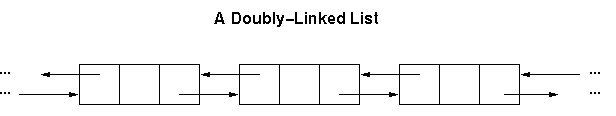
\includegraphics[scale=0.75]{images/linkedlist.png}
\label{fig: The Ranks and Files of a 4x4 Board}
\end{figure}
\end{center}
 To explain the core concept of Dancing Links, we'll first introduce the following functions. Suppose we have a doubly linked list with $x$ pointing to one of its elements. We define $L[x]$ and $R[x]$ to be a link pointing to the predecessor and successor of $x$, respectively. 
$$L[R[x]] \leftarrow L[x], \quad \quad R[L[x]] \leftarrow R[x]$$
We see above that in the left operation the predecessor of the successor of $x$, $L[R[x]]$, is assigned to the $L[x]$, thus removing $x$ from the list. Similarly in the right equation, the successor of the predecessor of $x$, $R[L[x]]$, is assigned to the $R[x]$, thus removing $x$ from the list. This is a simple backtracking operation that was well known before Knuth's paper, essentially we "cut out the middleman" to remove an unwanted element $x$. We call this operation \textbf{covering}. But what if we want to reintroduce $x$?
$$L[R[x]] \leftarrow x ,\quad \quad R[L[x]] \leftarrow x$$
In the left operation, the predecessor of the successor of $x$, $L[R[x]]$, is assigned to $x$ and similarly in the right operation, the successor of the predecessor of $x$, $R[L[x]]$, is assigned to the $x$. We simply undo the first set of operations, to "reintroduce the middleman" to recover $x$, so to speak. We call this operation \textbf{uncovering}. It seems intuitive given the first set of operations, but Knuth claims that these subtle operations were overlooked by many computer scientists at the time. He credits \cite{first} with the idea, who originally used these operations in an implementation of the N-Queens problem, which \textit{cut solving time almost in half} without adding a significant amount of complexity!
\subsection{How does Dancing Links improve efficiency?}
Dancing Links gives our algorithm the \textbf{depth-first backtracking} property. This means that the algorithm will not completely abandon the path, and will instead backtrack to the previous with multiple paths and continue from there. This is done by using the "covering" and "uncovering" operations to remove and reintroduce $x$. This property leads to quicker solve times as there are fewer nodes to be revisited.
\begin{figure}[ht]
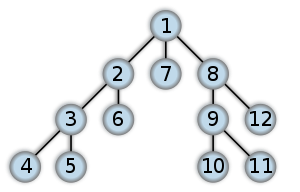
\includegraphics[scale=1]{images/depth-first.png}
\caption{Depth-first backtracking (source:Wikipedia)}
\label{fig: Depth-first backtracking (source:Wikipedia)}
\end{figure}
In this figure [...]
\clearpage
\section{The N-Queens Problem}
\subsection{Forming the 1-0 Matrix}
This general approach will be the first step toward solving the N-Queens problem. This matrix will be called the 1-0 matrix henceforth. The 1-0 matrix has a particular structure in the context of this problem, namely: The columns correspond to the satisfaction of the problem’s constraints, while the rows correspond to all the possible queen placements. For each placement, there will be a 1 for each satisfied constraint, and a 0 otherwise. Details of the constraints are discussed below, but first we must define the board and coordinates clearly.
In standard chess we refer to horizontal rows of the board as ranks, and vertical columns as files. Although in chess it is standard to begin counting at 1, in this context we will begin at 0 (We are using python after all).
Here we can see the ranks and files of a size n=4 chessboard:

\begin{center}
\begin{figure}[ht]
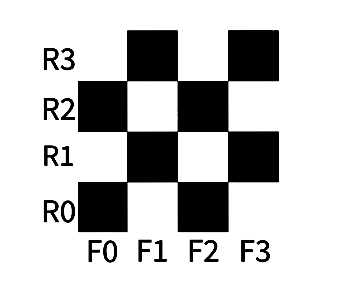
\includegraphics[scale=1]{images/chess1.png}
\caption{The Rank and File constraints}
\label{fig: The Ranks and Files of a 4x4 Board}
\end{figure}
\end{center}
Now we must discuss how this matrix is formed for a board of size n.

Speaking technically, we will not solve the actual problem using a matrix or NumPy array, instead we will create a set of doubly linked circular lists, running vertically and horizontally. However, it seems the most direct way to create this linked list, is to first create a NumPy array, with the 1s and 0s correctly filled, and then to convert it into a doubly linked circular list.

The columns of the 1-0 matrix correspond to the various constraints in the problem, namely two primary and two secondary constraints:
	Primary
	1.) There must be one and only one queen per rank.
	2.) There must be one and only one queen per file.
	Secondary
	3.) There can be at most one queen per diagonal.
	4.) There can be at most one queen per reverse-diagonal.
The rows of this matrix correspond to each of the possible queen placements, for example a queen at (0,0) or at (2,3). 

\subsection{Numbering the constraints}
It is worth noting here that we can disregard the four diagonals of length one, namely the two diagonals at points (0, n) and (n, 0) and the two reverse-diagonals at (0, 0) and (n, n). If a queen is occupying a diagonal of length one, it is simply not possible to have another queen occupy the same diagonal, therefore there is no need to ‘record’ whether or not such a constraint has been satisfied.

There are exactly 2n – 3 diagonals (and reverse-diagonals) on the board. 

Consider the uppermost rank on the board and the first file (the left and top edges), each square has one diagonal originating from it, and traversing the board toward the bottom right. This would give us a total of 2n diagonals, n for each side. We must subtract two for the aforementioned diagonals of length one, which originate in the corners, and also subtract an additional one for the ‘middle’ diagonal, which will be counted twice. This logic shows there are 2n-3 diagonals (and similarly 2n-3 reverse-diagonals).

It is helpful to number these constraints, as these numeric labels will correspond to the constraints (the columns) of the 1-0 matrix.
The rank constraints will be numbered 0,1, …, n-1.
The file constraints will be numbered n, n+1, …, 2n-1.
The diagonal constraints will be numbered 2n, 2n+1, …, 4n-4.
The reverse-diagonal constraints will be numbered 4n-3, 4n-3, …, 6n-7.

Below we can see a simple diagram illustrating these constraints for a n=4 chessboard.
The diagonals are coloured in blue, while the back diagonals are coloured in red.

\begin{figure}[ht]
\centering
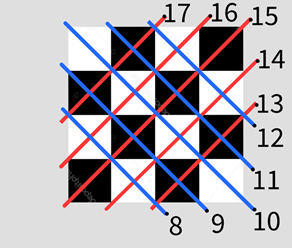
\includegraphics[scale=1]{images/chess2.png}
\caption{The Diagonal (Blue) and Reverse-Diagonal (Red) constraints}
\label{fig: The Diagonal (Blue) and Reverse-Diagonal (Red) constraints}
\end{figure}

Now we must discuss how this matrix is formed for a board of size n.
\subsection{A method for calculating the constraints}
Now we can calculate all the constraints which are satisfied by the various positions of queens:	
$$(i,j) \forall  i \geq 0 , j \leq n-1$$

We can see the python output for the case n=4 here, with the constraints roughly labelled following the outline specified before; ranks 0 through n-1, files 0 through n-1 then diagonals and reverse-diagonals. Along the rows we can see the various queen placements, first (0,0) through (0, n-1), then (1,0) through (1, n-1) and so on.

\begin{figure}[ht]
\centering
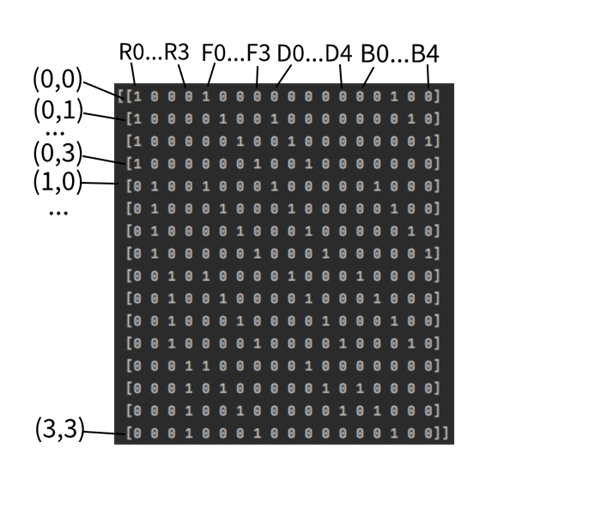
\includegraphics[scale=0.8]{images/chess3.png}
\caption{Labelled console output of the 1-0 matrix}
\label{fig: Labelled console output of the 1-0 matrix}
\end{figure}

\subsection{Conversion to a doubly linked list}
Three separate classes are used for the formation of this list, first a CircularList class, next a column class and lastly a node class.

The node class simply contains four attributes: up, down, left and right. These point to the other nodes around this node and will be used in the DLX algorithm to cover and uncover rows.
The column class contains the same four attributes as the node class, as well as two additional attributes: name and size. Name is a string which will allow humans to interpret which constraint this column represents (Rank 0 or Diagonal 3 for example), size is an integer which refers to the number of nodes or 1s, that are below a particular column header, and is used to select optimal rows during DLX.
The CircularList class contains only one attribute, a column object with the name ‘Master’, the entire list object will be built around this, and during DLX it will serve as a starting pointer to traverse the list. This master node lives left of the first column header, and as such the up, down and size attributes are not used.

 \begin{figure}[ht]
\centering
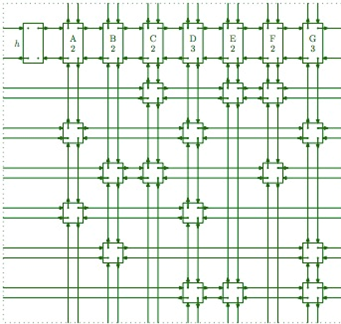
\includegraphics[scale=0.7]{images/chess4.png}
\caption{Illustration of a doubly linked circular list from Donald Knuth's Dancing Links paper}
\label{fig: Illustration of a doubly linked circular list from Donald Knuth's Dancing Links paper}
\end{figure}


\begin{verbatim}
A class specific function convert_one_zero , is used to convert the 1-0 matrix into a circular list object.
\end{verbatim}
\begin{verbatim}
Briefly in pseudocode:

	Repeat for each column of 1-0 matrix:
		Create column node
		Name column node
		Connect column node to the previous column node
	Repeat for each row of 1-0 matrix:
		Search the row
		If row[i] is 1:
			Create a node
			If not first node in row:
				Connect node.left to the previous node
			Find the corresponding column header
			Search until the bottom of this column/vertical list is found
				Connect below to node
	Repeat for each column:
		Traverse column to the bottom
		Update column.size accordingly
		Connect ‘lowest’ node.down to the header
		Connect header.up to the ‘lowest’ node	
	Connect furthest right column header.right to the master
	Connect master.left to the furthest right column header

This function converts the 1-0 matrix into a doubly linked circular list.
\end{verbatim}


\section{Collaboration Outline}
[not done]\\
Github, 
slack where we outlined collaborative goals, priorities, informal deadlines, 
weekly zoom meetings, 
work journal
...
\clearpage
\section{Conclusion}
\clearpage

\bibliographystyle{plain}
\bibliography{references}
\clearpage
\section{Appendices}
\clearpage
'''
\textbf{This page not for final script}\\
To do list:\\
rephrase commented sections\\
finish NP-Complexity section, add graph\\
check if there are any diagrams demonstrating properties of algorithm x\\
finish depth-first\\


\textbf{Format of manuscript: (From Blackboard)}

•Cover page

•Declaration page

•Introduction

•Main body (structured into sections as per topic requires).

•Collaboration Outline

•Conclusion 

•Bibliography

•Appendices (if applicable)

This page just for reference
'''
\end{document}
